\documentclass[]{article}
\usepackage{commons/course}
\usepackage{mathtools}
\DeclarePairedDelimiter\ceil{\lceil}{\rceil}
\DeclarePairedDelimiter\floor{\lfloor}{\rfloor}

\begin{document}
	
\begin{titlepage}
\begin{center}
\heading
\end{center}
\end{titlepage}
%%% title pages


%%% header of pages
\newpage
\pageheader
\tableofcontents

\newpage

 \Large \textbf{}
%%%
\begin{section-container}{شرح وظایف}
\end{section-container}


\pagebreak



\begin{section-container}{مقدمه}
	
	\subsection{تعریف الگوریتم}
	الگوریتم مورد استفاده الگوریتم ضرب ماتریسی \lr{Cannon} می‌باشد در این الگوریتم با تقسیم کردن ماتریس‌های ورودی و خروجی به بلاک‌های $k*k$ که در آن $k$ عدد ثابتی می‌باشد می‌خواهیم با داشتن تعدادی پردازنده‌ که به صورت موازی کار می‌کنند عملیات ضرب ماتریسی را بهبود ببخشیم. به طور مثال ماتریس‌ها زیر را در نظر بگیرید:
	\begin{equation}
	A = \begin{bmatrix}
	A_{11}& A_{12}& \dots A_{1\mu}\\
	\vdots& \ddots& \vdots\\
	A_{\lambda1}& A_{\lambda2}& \dots A_{\lambda\mu}\\
	\end{bmatrix} 
	\ \ \, 
	B = \begin{bmatrix}
	B_{11}& B_{12}& \dots B_{1\gamma}\\
	\vdots& \ddots& \vdots\\
	B_{\mu1}& B_{\mu2}& \dots B_{\mu\gamma}\\
	\end{bmatrix} 
	\end{equation}
	
	که در آن هر $A_{ij} و B_{ij}$ یک بلاک $k*k$ می‌باشد.(توجه می‌کنیم که  سایز‌ ماتریس‌ها اگر بخش‌‌پذیر به $k$ نباشد با اضافه‌ کردن صفر آن را بخش پذیر می‌کنیم) با این اوصاف طبق قاعده‌ی ضرب بلوکی می‌دانیم که بلاک $C_{ij}$ در ماتریس جواب از رابطه‌ی زیر محاسبه می‌شود.
	\begin{equation}
	C_{ij} = \sum_{x=0}^\mu A_{ix}B_{xj}
	\label{1}
	\end{equation}
	
	با داشتن تعداد تعداد مشخصی ضرب کننده‌ی ماتریسی $k*k$ می‌توانیم این به طور موازی با استفاده از آنها حاصل نهایی $A\times B$ را محاسبه کنیم. 
	
\end{section-container}

\subsection{قرارداد‌های ریاضی}

توجه می‌کنیم که در ادامه‌ی این گزارش و توضیحات لازمه در نظر می‌گیریم که ماتریس‌های ورودی $A_{mr}$ و $B_{rn}$ خواهند بود و بنابراین ماتریس‌ خروجی به صورت
$A_{mr} \times B_{rn} = C_{mn}$
خواهد بود. همچنین لازم است که توجه داشته باشید که وقتی ماتریس‌ها را به فرم بلوکی می‌نویسیم مقادیر زیر را تعریف می‌کنیم:
\begin{subequations}
	\begin{equation}
		\mu = \ceil*{\dfrac{r}{k}}
	\end{equation}    
	\begin{equation}
		\lambda = \ceil*{\dfrac{m}{k}}
	\end{equation}
	\begin{equation}
	\gamma = \ceil*{\dfrac{n}{k}}
	\end{equation}
\end{subequations}
از این نماد‌ها به کرّات در طول گزارش استفاده خواهد شد. توجه می‌کنیم که علت اینکه سقف این حاصل تقسیم‌ها را در نظر گرفتیم همان است که اگر اندازه‌ی ماتریس‌ها بر $k$ بخش‌پذیر نباشد با اضافه کردن صفر به انتها‌ی آن باعث بخش‌پذیری می‌شویم. 
\subsection{نحوه‌ی عملکرد از نظر مساحت و تایمینگ}
از آنجایی که هر ضرب کننده‌ی ماتریسی در حدود
 $k^3$
 کلاک سایکل زمان می‌برد و محاسبه‌ی هر بلوک $C_{ij}$ با توجه به
 \autoref{1}
به $\mu$ بار به ضرب ماتریسی نیاز دارد. همچنین برای محاسبه‌ی تمام بلوک‌ها باید $\lambda\gamma$ بار محاسبات بالا را انجام دهیم با این حال اگر فرض کنیم که تعداد پردازنده‌ها $p$ باشد آنگاه می‌توانیم ببینیم که تعداد کلاک‌ سایکل‌ها تقریبا برابر با عبارت زیر است:
\begin{equation}
	\dfrac{\lambda\gamma\mu k^2}{\text{\lr{\#number of PU}}} = 	\dfrac{\lambda\gamma\mu k^2}{p}
\end{equation}

\subsection{استاندارد‌ \lr{IEEE 754}}
محاسبات در این پروژه از استاندارد
 \lr{IEEE 754 - Single-precision floating-point}
 پیروی می‌کند که به طور مختصر به شرح آن می‌پردازیم. \\
 در این استاندارد اعداد اعشار با سه بخش \lr{exponent} , \lr{fraction} , \lr{sign} مشخص می‌شوند که سهم هر یک از آنها مانند مثال زیر است:
 
\begin{figure}[h]
	\centering
	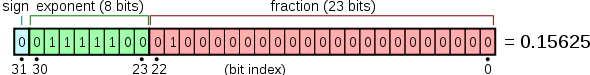
\includegraphics[width=0.8\linewidth]{source/float_example.png}
\end{figure}

و هر عدد طبق فرمول زیر به این نمایش در می‌آید:

\begin{equation}
\text{value} = (-1)^{sign} \times 2^{(E-127)} \times (1 + \sum_{i=1}^{23}b_{23-i}2^{-i})
\end{equation}
 
\subsection{مراجع مورد استفاده}

\pagebreak
\section{توصیف معماری سیستم}
\subsection{اینترفیس‌های سیستم و قرارداد استفاده از آن }
\subsection{دیاگرام‌های بلوکی سخت‌افزار}
\subsection{توصیف ماجول‌ها}
\subsection{ساختار درختی سیستم}

\pagebreak
\section{روند شبیه‌سازی و نتایج حاصل}
\subsection{توصیف \lr{TestBench}ها}
\subsection{توصیف روند کلی شبیه‌سازی}
\subsection{توصیف \lr{Golden Model}}
\subsection{مقایسه‌ی خروجی‌های نهایی با \lr{Golden Model}}



\end{document}







